\documentclass[a4paper]{article}
\usepackage[spanish]{babel}
\usepackage[utf8]{inputenc}
\usepackage{listings}
\usepackage{graphicx}
\graphicspath{ {./imagenes/} }

\lstset{
  frame=tb,
  language=Java,
  aboveskip=3mm,
  belowskip=3mm,
  showstringspaces=false,
  columns=flexible,
  basicstyle={\small\ttfamily},
  numbers=none,
  breaklines=false,
  breakatwhitespace=true,
  tabsize=1
}

\title{Practica 1 \newline \newline
	  \large \textbf{ Teoría computacional N, Profesor: Genaro Martinez} }

\author{\Large \textbf{Alumno:} \\ Luis Diego Jiménez Delgado \\ 
		\texttt{2CM5, luijsimenez6245@hotmail.com}}

\begin{document}
	\begin{titlepage}
		\maketitle
	\end{titlepage}
	{ \large \tableofcontents }
	\newpage
        \section{Cadenas Binarias}
        Tendencia de los números primos
        Objetivo del programa: Encontrar un patrón cuando se generan números primos en el intervalo (1,1000 000)
        Proceso: 
            \begin{itemize}
                \item Recibe un numero n <=1 000 000 y n>1
                \item Guarda los números primos desde n=1 hasta n
                \item Convierte los números a binario
                \item Se lee la cantidad de 1’s aparecen por número y se guarda esa cantidad por posición
                \item  Se representan estos resultados en una gráfica de posición contra cantidad de unos por número primo.
            \end{itemize}
                Se escogen los números que sean primos en un rango en el intervalo [2,n] donde n es un numero proporcionado por el usuario. Se aceptan los números dados sí y solo sí n>1, después se verifica que desde 2 hasta n no existan números que dividan a n, es decir, el número módulo i (número dentro del rango), tiene que ser distinto de cero excepto cuanto i es igual al número.
                Segunda etapa: Los números se convierten a binario usando recursividad cuyo caso base es cuando el valor del número es menor a 2 y en el caso recursivo se envía el número divido entre dos.
                Tercera etapa: Para cada número generado se realiza un conteo de las ocurrencias del número 1 y se les asigna una posición por número. Estos datos se salvan en un archivo y posteriormente se grafican.
                Se obtiene una conclusión: este método no puede generalizarse para encontarr tendencia en los números primos, debido a que no parece tener un patro en el intervalo 1 - 1,000,000.
            \subsection{Espaciadas}
            Para el problema anterios se generó un archivo que contiene las cadenas divididas por un ENTER entre cada una de ellas, aplicando cuando n = 27, generado así un aproximado de 134, 217, 728 lineas y se almacena en un archivo de texto ``spaces.txt''.
            \begin{lstlisting}
#include <stdio.h>
#include <math.h>
#include <stdlib
void getWord(int length, int number);
FILE *fp;
int main(int argc, const char** argv)
{
    char * file_name = "/Volumes/FILES/files/spaces.txt";
    int n = 27, i, counter, j;
    if(argc == 2){
        n = atoi(argv[1]); 
    }
    fp = fopen (file_name, "wb");
    fclose (fp);
    fp = fopen (file_name, "ab");
    for (i = 0; i <= n; ++i)
    {
        counter = (int) pow(2, i + 1);
        printf("item: %d \n", i);
        for (j = 0; j < counter; ++j)
        {
            getWord(i, j);
        }
    }
    fclose (fp);
    return 0;

void getWord(int length, int number)
{
    char res[length + 2];
    res[length + 1] = '\n';
    res[length + 2] = '\0';
    int i, aux;
    for (i = length; i >= 0; --i)
    {
        aux = number >> i;
        if (aux & 1)
            res[i] = '1';
        else
            res[i] = '0';
    }
    fputs(res, fp);
}
            \end{lstlisting}
            Gráfica de 1's.
            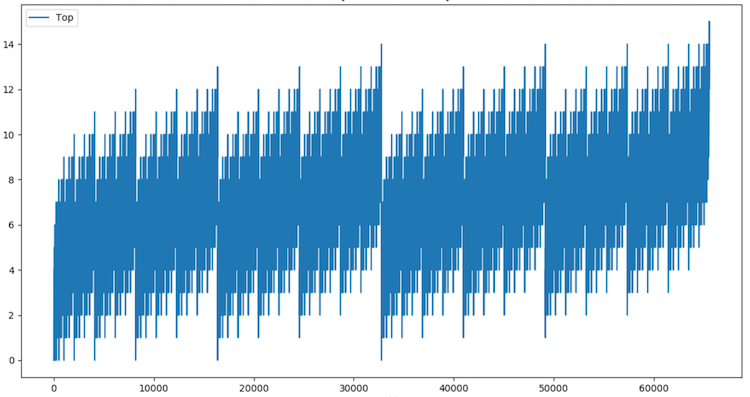
\includegraphics{File3}

            \subsection{Juntas}
            Se generó un archivo que contiene las cadenas sin separación alguna, generado así un archivo ``nospaces.txt'', aplicando el mismo caso anterior.
            \begin{lstlisting}
#include <stdio.h>
#include <math.h>
#include <stdlib.h>

void getWord(int length, int number);

FILE *fp;

int main(int argc, const char** argv)
{
    char * file_name = "/Volumes/FILES/files/no.txt";
    int n = 27, i, counter, j;
    if(argc == 2){
        n = atoi(argv[1]); 
    }
    fp = fopen (file_name, "wb");
    fclose (fp);
    fp = fopen (file_name, "ab");
    for (i = 0; i <= n; ++i)
    {
        counter = (int) pow(2, i + 1);
        printf("item: %d \n", i);
        for (j = 0; j < counter; ++j)
        {
            getWord(i, j);
        }
    }
    fclose (fp);
    return 0;
}

void getWord(int length, int number)
{
    char res[length + 1];
    res[length + 1] = '\0';
    int i, aux;
    for (i = length; i >= 0; --i)
    {
        aux = number >> i;
        if (aux & 1)
            res[i] = '1';
        else
            res[i] = '0';
    }
    fputs(res, fp);
}
            \end{lstlisting}
            
            Gráfica de 1 de cadenas de 16 bits.\newline
            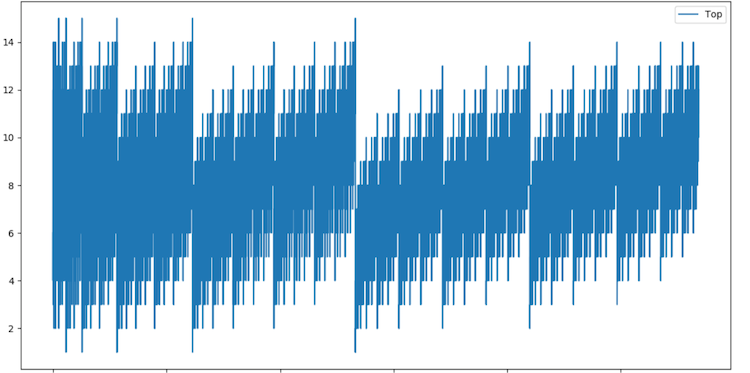
\includegraphics{File2}
            Gráfica de 1 de cadenas de 8 bits.\newline
            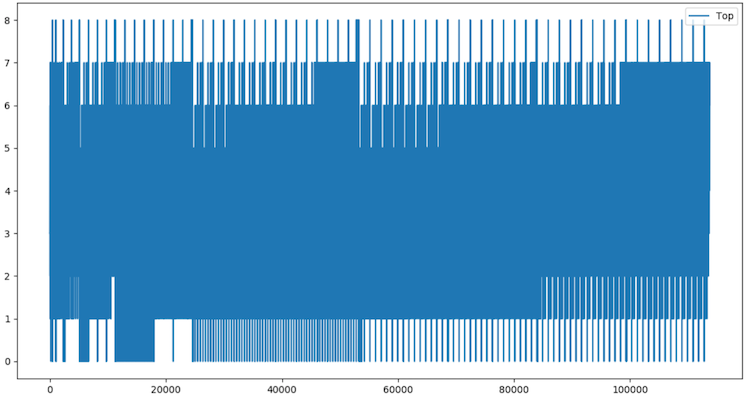
\includegraphics{File1}

            \subsection{Numeros Primos}
            Por medio de un algortimo básico para veirificar si un número era primo o no, se generó un archivo con todos lo números primarios del 2 - 100000 guardandolos en un archivo de texto de nombre ``prime.txt''
            Del cual se obtuvo el siguiente analisis:

            \begin{lstlisting}
#include <stdio.h>
#include <math.h>
#include <stdlib
void getWord(int length, int number);
int isPrime(int number);
FILE *
int main(int argc, const char **argv)
{
    char *file_name = "/Volumes/FILES/files/prime.txt";
    int n = 100000, i, counter, j = 1;
    if (argc == 2)
    {
        n = atoi(argv[1]);
    }
    fp = fopen(file_name, "wb");
    fclose(fp);
    fp = fopen(file_name, "ab");
    for (i = 2; i <= n; ++i)
    {
        if((i % (10*j)) == 0)
        {
            j += 1;
        }
        if(isPrime(i))
        {
            getWord(j, i);
        }
    }
    fclose(fp);
    return 0;

int isPrime(int number)
{
    int i = 2, res = 1;
    for(i = 2; i <= number/2; ++i)
    {
        if((number%i) == 0)
        {
            res = 0;
            break;
        }
    }
    return res;

void getWord(int length, int number)
{
    char res[length + 2];
    res[length + 1] = '\n';
    res[length + 2] = '\0';
    int i, aux;
    for (i = length; i >= 0; --i)
    {
        aux = number >> i;
        if (aux & 1)
            res[i] = '1';
        else
            res[i] = '0';
    }
    fputs(res, fp);
}
            \end{lstlisting}
            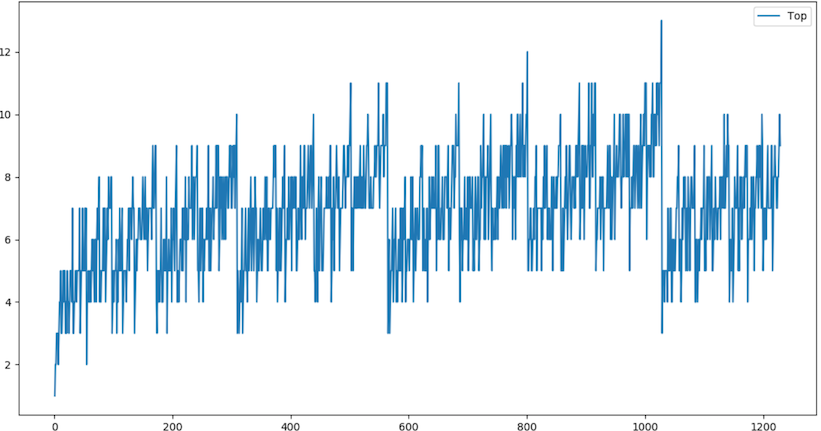
\includegraphics{File4}

        \section{Buscador de ANSI C}
            El proposito de programa es realizar un automata capaz de identificar todas las palabras reservadas de ANSI extraerlas y en un archivo guardar en donde se encunetran y el númrero de repeticiones que hay en el texto de entrada.
            \begin{itemize}
                \item El autómata comienza con cualquier caracter de entrada.
                \item Cuando el automata encuentra un cáracter diferente a un espacio o salto de linea el programa comienza a busacr en el diccionario que tiene almacenado con las palabras reservadas.
                \item Va verificando caracter por caracter para ver que sea una palabra correcta, indentifica todos los caracteres al igual que distingue de mayúsculas y minúsculas.
                \item Almacena las palabras que guardo
                \item Genera un archivo para visualizar los resultados.
            \end{itemize}
            Se realizó otro automata para visualizar el proceso de este de manera gráfica representado por nodos.
            \begin{lstlisting}
import os
from os.path import isfile, join
import json 

rdic = dict()

def evaluate(c, position, dictionary):
    res = list()
    for word in dictionary:
        l = list(word)
        if not (len(l) <= position):
            if l[position] == c:
                res.append(word)
    return res

def create_existing_item(word, index, line):
    if word in rdic:
        rdic[word] += 1
    else: 
        rdic[word] = 1
    return "{\"linea\":"+str(line)+",\"caracter\": " + str(index -  len(word))+ ", \"word\":\"" + str(word)+"\"}"

def scope(dictionary, text):
    is_posible = True
    possible_words = dictionary
    counter = 0
    index = 0
    line_counter = 0
    word = ""
    res =  ""
    lines = text.split("\n")
    for line in lines:
        index = 0
        for item in line:
            if(item == " " or item == "\n" or item == "\t" or item == "\0"):
                counter = 0
                if(is_posible) and index != 0 and word in dictionary:
                    res +=  create_existing_item(word, index, line_counter) + ","
                word = ""
                possible_words = dictionary
                is_posible = True
            elif(is_posible):
                word += item
                possible_words = evaluate(item, counter, possible_words)
                is_posible = (len(possible_words)!= 0)
                if(is_posible):
                    counter += 1 
            index += 1
        line_counter += 1
    return res[:-1]


def read_file(path):
    res = ""
    with open(path) as fp:
        line = fp.readline()
        while line:
            res += line
            line = fp.readline()
    return res


def write_file(name, content):
    if(os.path.isfile(name)):
        pass
    f = open(name, "w+")
    f.write(content)
    f.close()
    return

if __name__ == "__main__":
    file_content = read_file("dic.txt")
    dictio = file_content.split("\n")
    document = read_file("./program.c")
    r = scope(dictio, document)
    r = "{\"items\": ["+ r +"]," +  "\"repeticiones\" : " + json.dumps(rdic) + "}"

    write_file("./res.json", r)                
            \end{lstlisting}
            Modelo de autómata funcional en caso particular.\newline
            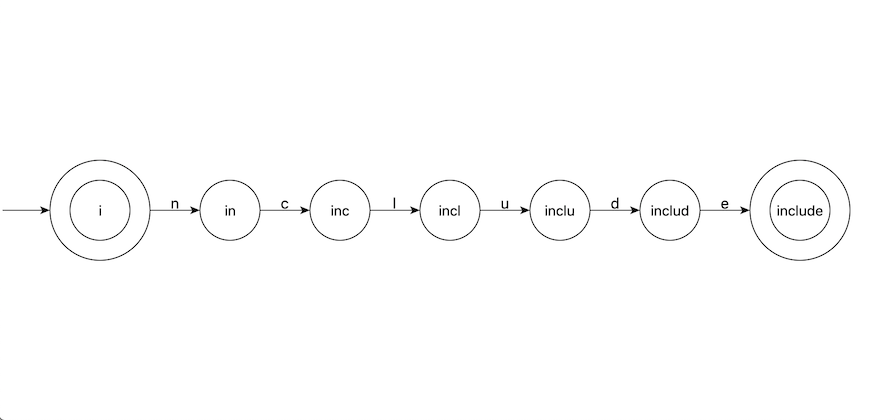
\includegraphics{auto}
            Modelo de autómata funcional en caso particular no valido.\newline
            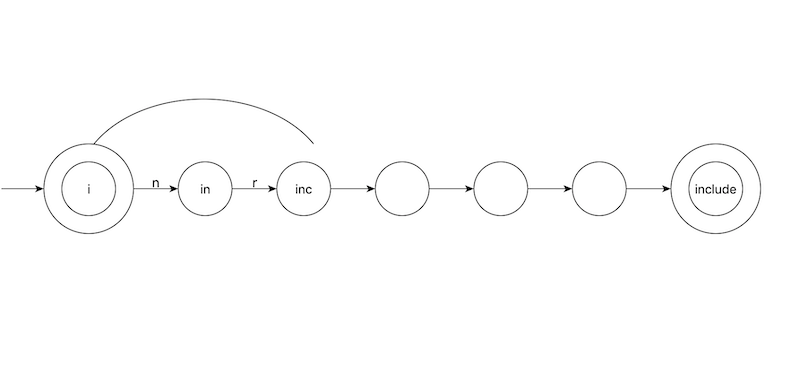
\includegraphics{autoM}

		\section{Automata de cadenas}
			En este programa se verifican a través de un autómata las cadenas de que simulan ser transacciones y consiste en lo siguiente: 
			\begin{itemize}
                \item El autómata comienza si tiene un número aleatorio que 
                \item Se generan los datos de entrada.
                \item Se hace la lectura de las cadenas generadas.
                \item En el bloque ACK se generan dos archivos 
                \item  Se genera un número aleatorio entre 0 y 1 (inclusive), y se regresa al paso 1. 
            \end{itemize}
            Para comenzar con la explicación del automata, pirmero se debe de generar un número aleatorio entre 0 y 1 que nos indicará si el autómata comienza o no.
            Se crea una cadena de 100000 caracteres que se envia solo si el otro automata está encendido o no.
            Si el segundo está encendido, recibe la cadena generada y valida que sea una cadena de 1000000 caracteres, y que su valor en binario sea impar. 
            En caso de que tengan paridad se crea un archivo ``accepted.txt'' (véase la figura 3), el cual contiene la cantidad de cadenas aceptadas y el número de proceso en el que se encontraron. 
            En el otro caso, se crea un archivo ``unaccepted.txt'' (véase la figura 4), el cual contiene la cantidad de cadenas rechazadas y el número de proceso en el que se encontraron. 
            Luego, se tiene un archivo ``history.txt'' (véase la figura 5 y 6), el cual nos indica el estado del autómata por proceso, y finalmente se genera otro número aleatorio que nos indicará si nuevos datos van a entrar o el programa finaliza. 
            
            \begin{lstlisting}
from random import randint

class Receiver():

    def __init__(self):
        pass

    def is_active(self):
        return ((randint(0, 2) % 2) == 0)
    
    def recieve_word(self, word):
        return self.verify_word(word)

    def verify_word(self, word):
        one = 0
        cero = 0
        for item in word:
            if(item == "1"):
                one += 1
            else:
                cero += 1 
        return cero%2==0 and one%2==0
            \end{lstlisting}
            \begin{lstlisting}
from random import randint
                
class Receiver():
                
    def __init__(self):
        pass

    def is_active(self):
        return ((randint(0, 2) % 2) == 0)
    
    def recieve_word(self, word):
        return self.verify_word(word)

    def verify_word(self, word):
        one = 0
        cero = 0
        for item in word:
            if(item == "1"):
                one += 1
            else:
                cero += 1 
        return cero%2==0 and one%2==0
                            \end{lstlisting}
                            \begin{lstlisting}
import Sender
import Receiver

if __name__ == "__main__":
    res = Sender.Sender(open("./history.text", "w+"), open("./accepted.txt", "w+"), open("./unaccepted.txt", "w+"))
    res.enable(Receiver.Receiver())
    print(res.times)
    res.history.close()
    res.accepted.close()
    res.unaccepted.close()
                                            \end{lstlisting}
        \section{Graficadores}
            Por último se agregan 2 de las herramientas que se utilizaron para mostrar als imagenes presentadas en el reporte
            \subsection{Graficadora de elementos}
            Se graficó por medio de algunas librerías de python realizando de manera gráfica la cantidad de 1's que había en la respectiva cadena
            \begin{lstlisting}
import files as Files
import numpy as np
from plotly.offline import download_plotlyjs, init_notebook_mode, plot
from plotly.graph_objs import *
import plotly.graph_objects as go
import math
from IPython.display import display, HTML
import sys


file_name =  '/Volumes/FILES/name2.html'
fi = Files.read_file("/Volumes/FILES/res-test")  
fi = fi[:-1]
items =  fi.split("\n")

to_work_x = list()
to_work_y = list()

i = 0
for item in items:
    aux = len(item.replace("0",""))
    to_work_x.append(aux)
    to_work_y.append(i)
    i = i +1


colorVector = "rgb(84,128,5)"
colorR = "rgb(84,11,5)"

lineDictV = dict( 
                color = colorVector,
                width = 6
            )
lineDictR = dict( 
                color = colorR,
                width = 6
            )
markerV = dict( size = 1,
            color = colorVector)

markerR = dict( size = 1,
            color = colorR)

layoutMargin = dict( 
            l = 0,
            r = 0,
            b = 0,
            t = 0
        )



layout = Layout(
        margin = layoutMargin,
        xaxis=dict(
            autorange = True,
        ),
        yaxis=dict(
            autorange = True,
        )
    )  

fig= go.Figure(data=go.Scatter(x= to_work_y, y=to_work_x))
plot(fig, filename=file_name, auto_open=False)

print(file_name)

            \end{lstlisting}
                
            \subsection{Graficadora de automatas}
            Se graficó por medio de algunas librerías de python realizando circulos y lineas para visualizar mejor el automata del ejercicio del Automata de Cadenas
            \begin{lstlisting}
#Panel.py
from tkinter import Tk, Canvas, Frame, BOTH
import math
                
class Panel(Frame):
                
    canvas = None
    width_stroke = 1
    fill = "#ffffff"
    outline = "#000000"

    def __init__(self, title = ""):
        super().__init__()
        self.canvas = Canvas(self)
        self.pack(fill=BOTH, expand=1)
        self.canvas.pack(fill=BOTH, expand=1)
    
    def add_arc(self, position_x, position_y, t0, t1):
        return canvas.create_arc(x-r, y-r, x+r, y+r, start=t0, extent=t1-t0,style='arc', width=self.width_stroke)    

    def add_circle(self, x, y, text = "", r = 40):
        diameter = r / 2
        self.canvas.create_oval(x+r, y+r, x-r, y-r, width=self.width_stroke)
        if(text !=  ""):
            self.add_text(x , y , text= text, font_size = math.ceil((r - 10) * 2 /3))
        self.canvas.update()
    
    def add_arrow(self, points):
        return self.canvas.create_line(points, width = self. width_stroke)
        
    def add_elliptical_arc(self,x, y, r1, r2, t0, t1, start_arrow=1, end_arrow=0):
        return self.canvas.create_arc(x-r1, y-r2, x+r1, y+r2, start=t0, extent=t1-t0, style='arc', width= self.width_stroke)

    def add_line(self, x1, y1, x2, y2, start_arrow=0, end_arrow=0, text = "s", font_size = 15):
        arrow_opts = start_arrow << 1 | end_arrow
        arrows = {0b10: 'first', 0b01: 'last', 0b11: 'both'}.get(arrow_opts, None)
        if(text !=  ""):
            self.add_text(x1 + (x2-x1)/2, y1 -(font_size/2), text= text, font_size = font_size)
        return self.canvas.create_line(x1, y1, x2, y2, width=self.width_stroke, arrow= arrows)

    def add_text(self, x, y, text, font_size = 15):
        return self.canvas.create_text(x, y, text=text, font=('bold', font_size))
        \end{lstlisting}
            \begin{lstlisting}
#app.py
from tkinter import Tk, Canvas, Frame, BOTH
from Panel import Panel
class Coordinate():
    x = 0
    y = 0
    def __init__(self, x, y):
        self.x  = x
        self.y = y
    
def main():
    root = Tk()
    panel = Panel()
    width = 0
    heigth = 420 
    parent = create_main_node(panel, Coordinate(x = 0, y = 0), "q0", heigth)
    r = parent
    dic = {("q1", "1"), ("q2","cadena"), ("q3", "es valida")}
    for item in dic:
        r = create_node(panel, r, item)
    final = create_main_node(panel, r, "qf", heigth)
    node_to_node(panel, final, parent, 1)
    width = final.x
    width += 50
    root.geometry( str(width) +"x"+ str(heigth) +"+300+300")
    root.mainloop()
def create_main_node(panel, coordinate, state, heigth):
    middle_heigth = (heigth/2)
    r = create_double_node(panel, Coordinate(x = coordinate.x + 100, y = middle_heigth), state)
    panel.add_line(coordinate.x,  middle_heigth, coordinate.x + 50,  middle_heigth, end_arrow=1)
    return r
def create_double_node(panel, coordinate, state):
    panel.add_circle(coordinate.x, coordinate.y, "", 50)
    panel.add_circle(coordinate.x,  coordinate.y, state, 30)
    return Coordinate(x = coordinate.x + 50, y = coordinate.y)
def create_node(panel, coordinate, state, changing_state = ""):
    width = 30
    res =  Coordinate(x = coordinate.x + 20 + (width * 2), y = coordinate.y)
    panel.add_line(coordinate.x, res.y, res.x - width, res.y, end_arrow=1)
    panel.add_circle(res.x, res.y, state, width)
    res.x += width
    return res
def node_to_node(panel, coordinate_self, coordinate_to, radio_self, radio_to = 0):
    if radio_to == 0:
        radio_to = radio_self
    mid_x = (coordinate_self.x + (coordinate_to.x /3) ) /2
    mid_y = coordinate_self.y  
    panel.add_elliptical_arc(mid_x, mid_y, coordinate_self.x - mid_x, 100, 30, 180-30)
    pass
if __name__ == '__main__':
    main()
        \end{lstlisting}
\end{document}  